\documentclass[12pt, letterpaper, twoside]{article}
\usepackage[utf8]{inputenc}
\usepackage{graphicx}

\author{Charlie Crisp, Pembroke College }
\date{October 2017}

\newcommand{\horrule}[1]{\rule{\linewidth}{#1}} % Create horizontal rule command with 1 argument of height

\title{	
	\normalfont \normalsize 
	\textsc{Computer Science Tripos - Part II - Project Proposal} \\ [25pt]
	\horrule{0.5pt} \\[0.4cm] % Thin top horizontal rule
	\huge Building a Blockchain Library for OCaml\\ % The assignment title
	\horrule{2pt} \\[0.5cm] % Thick bottom horizontal rule
}

\date{\normalsize\today} % Today's date or a custom date

\begin{document}
	
	\maketitle
	
	\noindent \textbf{Project Supervisor:} KC Sivaramakrishnan \\
	\textbf{Director of Studies:} Anil Madhavapeddy \\
	\textbf{Project Overseers:} Timothy Jones \& Marcelo Fiore\\
	
	\section*{Introduction}
	
	The blockchain, in its simplest form, is a tree-like data structure. Chunks of data are stored in 'blocks' which contain the hash of the contents of the previous block. This creates a 'blockchain' which can exhibit branching in the same way that a tree data structure can (see Figure \ref{fig:blockchain}). One of the most important features of a blockchain, is that a change in a block, will alter the block's hash, thereby altering all the future blocks in the chain. This makes it very easy to validate that the data in a blockchain is trustworth, by verifying the hash in a block, is the same as the hash of it's parent's content.
	\begin{figure}
		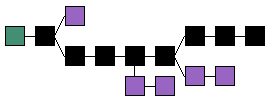
\includegraphics[width=\linewidth]{blockchain}
		\caption{A typical blockchain structure \cite{Blockchain Image}}
		\label{fig:blockchain}
	\end{figure}
	\\
	\noindent Blockchain technology has generated a lot of interest in recent times, but mostly in the field of cryptocurrencies.
	With a simple Proof of Work consensus algorithm, the blockchain can be used to build a secure, distributed ledger of transactions. However, whilst the uses of the blockchain are far wider reaching than cryptocurrencies, progress outside of this field has been much slower. 

	\noindent I will build a pure OCaml, reusable blockchain library to allow the creation of distributed, secure ledgers, which are agreed upon by consensus. The library will allow users to create and add entries to a distributed blockchain ledger with just a few lines of code. The users will also be able to trust that entries in the blockchain are exactly replicated across all nodes in the network.

	\noindent It will be built on top of Irmin \cite{Irmin} - a distributed database with git-like version control features. Being pure OCaml, the blockchain nodes can be compiled to unikernels or JavaScript to run in the browser. I will evaluate the blockchain by prototyping a decentralised lending library and evaluating the platform’s speed and resilience.
	\section*{Starting point}
	The project will build upon functionality provided by Irmin \cite{Irmin} which is a distributed database system. 
	Irmin is fast, durable and has the branching capabilities which are required to build a blockchain.

	\section*{Resources required}
	I will be using a Macbook provided by OCaml Labs \cite{OCaml Labs} in order to develop the source code for the project. If the Macbook fails, then I will easily be able to transfer my work onto the MCS machines, as my project has no special requirements. \\
	My work will also be backed up to a git repository hosted on GitHub and saved to a dedicated memory stick on a daily basis. \\
	During the evaluation stage I will be running my platform on different cloud based devices and/or Raspberry Pi's. There are many possible providers for cloud computing, including Amazon Web Services and Microsoft Azure. OCaml Labs \cite{OCaml Labs} will provide the necessary funds to acquire these resources.
	

	
	\section*{Background}
	\subsection*{Consensus}
	\noindent Consensus is a group process where a network of nodes will reach a general agreement. There are different ways of achieving consensus but here are some of the most common:
	\begin{enumerate}

	\item \textbf{Proof of Work}: Trust is given to nodes which can prove that they have put in computational work. This is the consensus mechanism used by Bitcoin.
	\item \textbf{Proof of Stake}: Nodes are selected to validate blocks based on their stake in the blockchain. There are few variations on this algorithm which introduce notions such as delegation or anonymity.
	\item \textbf{Raft Consensus}: A leader is elected and acts as a governing authority until it fails or disconnects, whereupon a new leader is elected.
	\end{enumerate}

	\section*{Work to be completed}
	The work for this project will be split into the following major parts.
	\begin{enumerate} 
		\item Design and build a module to allow nodes to create and maintain a blockchain ledger. This will include allowing nodes to add blocks to the chain and to form new branches.
		\item Design and build a module to allow nodes to interact over a network and to achieve consensus. As highlighted the Background section, there are many different ways to achieve consensus, and a large part of this work will be to determine which method is most suitable. This decision will take into account a method's failure tolerance in terms of nodes failing and network failure, as well as general speed and any requirements (e.g. computational work for a Proof of Work algorithm).
		\item Design an application using these modules. This will take the form of a book lending platform where nodes will be able to register books and lend them to other nodes in the network. This application has been chosen, because the blockchain library should allow for typically centralised applications to be created in a decentralised way. It will also allow for testing of critical features, for example, books should never be 'doubly-spent', i.e. if one user believes they have ownership of a book, then no other user will think the same.
		\item Design an evaluation program to simulate different load on the lending platform. This will be run in different configurations in order to measure the performance of the platform.
	\end{enumerate}
	\section*{Evaluation metrics and success criteria}
	I will consider the project to be a success if the following criteria are achieved:
	\begin{enumerate}
		\item Nodes in the network are able to connect and communicate information.
		\item Nodes are able to achieve consensus about the state of the distributed ledger.
		\item Nodes are able to reconnect after being individually disconnected.
		\item Nodes are able to re-converge after a network partition.
	\end{enumerate}
	In order to evaluate the performance of the system, I will measure the \textit{throughput} and \textit{speed} of transactions of the book lending platform. Throughput will be measured in transactions per second, and speed will be quantified as time taken to complete a transaction. I will evaluate how these properties vary with respect to the following metrics:
	\begin{enumerate}
		\item \textbf{Number of nodes}: I will scale the number of nodes in the network between the range of 2 and 5.
		\item \textbf{Rate of transactions}: I will vary the number of transactions made per second.
	\end{enumerate}
	Should I achieve and be able to measure the above criteria within the time frame of my project, I will further test system against the following metrics:
	\begin{enumerate}
		\item \textbf{Network latency between nodes}
		\item \textbf{Network bandwidth of nodes}
	\end{enumerate}
	\section*{Timetable}
	\begin{enumerate}
		\item \textbf{Michaelmas Weeks 2-4} (12/10/17 - 01/11/17):\\
		Set up an environment for developing OCaml and familiarise myself with the language and it's module system. This is important because the blockchain library needs to be reusable, and therefore well isolated.
		\item \textbf{Michaelmas Weeks 5-6}  (02/11/17 - 15/11/17):\\
		Familiarise myself with Irmin and it's data structures. This is important as I have never used the library before, but it will be used to build the blocks in the blockchain library. In this time I will also begin to design the API of my library.
		\item \textbf{Michaelmas Weeks 7-8} (16/11/17 - 29/11/17):\\
		Finalise the API and start to build the module for creating and interacting with a distributed ledger.
		\item \textbf{Christmas Vacation} (30/11/17 - 17/01/18):\\
		Finalise the API of the module for achieving consensus between multiple nodes. This work will also include investigating different methods of consensus and their suitability for my project.
		\item \textbf{Lent Weeks 1-2} (18/01/17 - 31/01/18):\\
		Build the module for achieving consensus between modules. I will also start work on an lending library application which will be used to evaluate the performance of the blockchain library. 
		\item \textbf{Lent Weeks 3-4} (01/02/18 - 14/02/18):
		\\
		Finish work on the lending library application and install it on a number of Raspberry Pi and/or cloud based devices. I will also begin work on my dissertation and I aim to complete the Introduction and Preparation chapters.
		\item \textbf{Lent Weeks 5-6} (05/02/18 - 28/02/18):\\
		Evaluate the performance of the platform by simulating load from each of the devices and measuring the speed of transactions. A stretch goal for this period is also to evaluate a range of further metrics. Additionally I will continue work on my dissertation and aim to complete the Implementation chapter.
		\item \textbf{Lent Weeks 7-8} (01/03/18 - 14/03/18):\\
		Finish a first draft of my the dissertation by writing the Evaluation and Conclusion chapters. I will also send the dissertation to reviewers to get feedback.
		\item \textbf{Easter Vacation} (15/03/18 - 25/04/18):\\
		With a first draft of the dissertation completed, I will use this time to review the draft and to make improvements. I will also incorporate feedback from reviewers, and complete the Bibliography and Appendices chapters.
		\item \textbf{Easter Weeks 1-2} (26/04/18 - 09/05/18):
		\\
		Conclude work on dissertation by incorporating final feedback from reviewers.
		\item \textbf{Easter Week 3-Submission Deadline} (10/05/18 - 08/05/18):\\
		I aim to have completed the dissertation by this point, and to be focusing on my studies. However, this time may be needed to make any final changes.
	\end{enumerate}
	\begin{thebibliography}{9}
		\bibitem{Irmin} 
		Irmin - A pure OCaml, distributed database that follows the same design principles as Git.\\ \textbf{https://github.com/mirage/irmin}
		\bibitem{OCaml Labs}
		OCaml Labs - An initiative based in the Computer Laboratory to promote research, growth and collaboration within the wider OCaml community\\
		\textbf{http://ocamllabs.io/}
		\bibitem{Blockchain Image}
		Image of blockchain data structure from Wiki Commons.
		\textbf{https://commons.wikimedia.org/wiki/File:Blockchain.png}
		
	\end{thebibliography}

\end{document}